%%% Meetup PostgreSQL Paris

\documentclass{beamer}

\usepackage[utf8]{inputenc}

\usepackage{beamerthemesplit}
\usetheme{Boadilla}
\setbeamertemplate{itemize items}{\checkmark}
%\setbeamertemplate{itemize items}[circle]
\beamertemplatetransparentcovered

\usepackage{multicol}

\title{PostgreSQL Meetup}
\subtitle{Paris}
\author{Dimitri Fontaine \texttt{dimitri@2ndQuadrant.fr}}
\date{8 Avril 2014}
\logo{
\includegraphics[height=0.4cm]{2ndQuadrant-cross.png}}

\begin{document}

\frame{\titlepage}

\begin{frame}[fragile]
  \frametitle{PostgreSQL Meetup}

  \begin{center}
    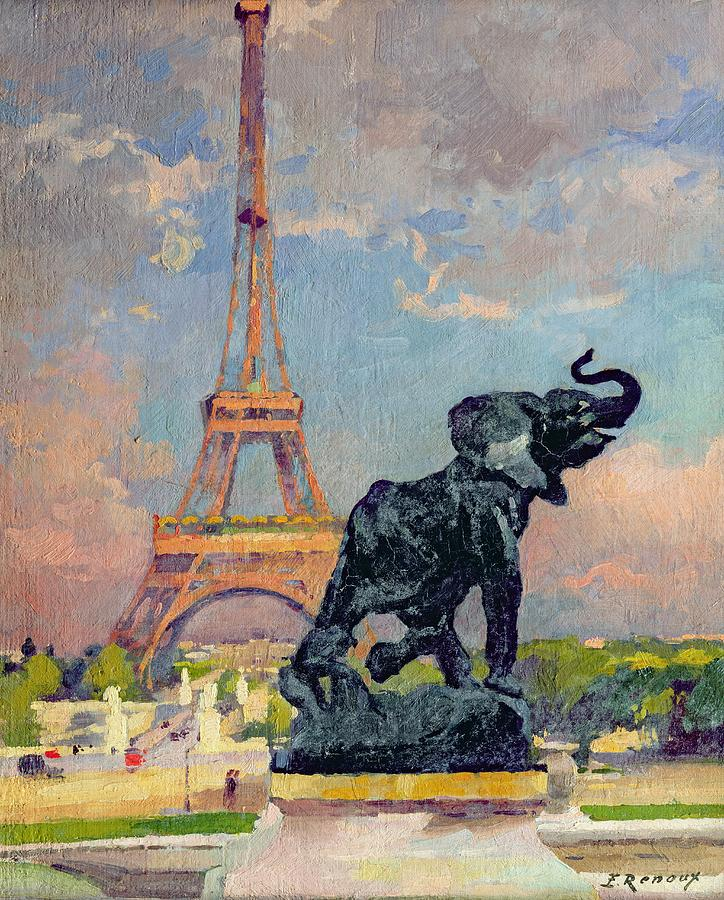
\includegraphics[height=18em]{the-eiffel-tower-and-the-elephant-by-fremiet-jules-ernest-renoux.jpg}
  \end{center}
\end{frame}

\begin{frame}[fragile]
  \frametitle{Financement par des sponsors}

  \center{Pour le lieu, merci \textbf{Mozilla}}
  \vfill
  
  \begin{center}
    
\includegraphics[height=12em]{logo_firefox.png}
  \end{center}
\end{frame}

\begin{frame}[fragile]
  \frametitle{Financement par des sponsors}

  \center{Pour le buffet, merci \textbf{Violin Memory}}
  \vfill
  
  \begin{center}
    
\includegraphics[height=9em]{VMLogoPMS.eps}
  \end{center}
\end{frame}

\begin{frame}[fragile]
  \frametitle{pgDay Paris, le 8 avril prochain}

  \begin{center}
    
\includegraphics[height=21em]{pgdayparis.png}
  \end{center}
\end{frame}

\begin{frame}[fragile]
  \frametitle{pgDay Paris}

  \center{Code promo \Large \textsc{\textbf{\textcolor{magenta}{MEETUP8}} -10\%}}
  \vfill
  
  \begin{center}
    
\includegraphics[height=15em]{pgdayparis.png}
  \end{center}
\end{frame}

\frame{
  \frametitle{Aujourd'hui}

  \center{Présentations de ce soir}
  
  \begin{itemize}
  \item \textit{Logical Decoding Plugin} by \textbf{Daniel Gustafsson}
  \item \textit{Modern SQL} par \textbf{Markus Winand}
\end{itemize}}
}

\end{document}
